\documentclass{article}

\usepackage[most]{tcolorbox}
\usepackage{physics}
\usepackage{graphicx}
\usepackage{float}
\usepackage{amsmath}
\usepackage{amssymb}


\usepackage[utf8]{inputenc}
\usepackage[a4paper, margin=1in]{geometry} % Controla los márgenes
\usepackage{titling}

\title{Clase 19 }
\author{Manuel Garcia.}
\date{\today}

\renewcommand{\maketitlehooka}{%
  \centering
  \vspace*{0.05cm} % Espacio vertical antes del título
}

\renewcommand{\maketitlehookd}{%
  \vspace*{2cm} % Espacio vertical después de la fecha
}

\newcommand{\caja}[3]{%
  \begin{tcolorbox}[colback=#1!5!white,colframe=#1!25!black,title=#2]
    #3
  \end{tcolorbox}%
}

\begin{document}
\maketitle

\section{Transporte paralelo y geodésicas }
\caja{red}{Ecuacion de las geodésicas }{
  \begin{gather*}
    \grad_V V = 0 \quad \rightarrow \quad \frac{d ^2 x^\mu  }{d t^2 } + \Gamma _{\nu \lambda } ^ {\mu } \frac{d x ^ {\nu } }{d t } \frac{d x ^ {\lambda} }{d t } = 0  
  \end{gather*}
}
Podemos relajar la condición $ \grad_V V = 0  $ por la condicion $ \grad _V V = fV  $, donde $ f \in \mathbb{F}(M)  $ 
\begin{gather*}
  \grad_V V = 0 \quad \rightarrow \quad \frac{d ^2 x^\mu  }{d t^2 } + \Gamma _{\nu \lambda } ^ {\mu } \frac{d x ^ {\nu } }{d t } \frac{d x ^ {\lambda} }{d t } = f \frac{d x ^ {\mu } }{d t }
\end{gather*}

\section{Derivada covariante de tensores }
\caja{red}{}{
  \begin{gather*}
    \grad _\alpha T _{\nu_1\cdots v_q } ^ {\mu_1 \cdots \mu_p } \equiv T _{\nu _1 \cdots v_q;\alpha }  ^ {\mu_1 \cdots \mu_p } = \frac{\partial T _{\nu_1 \cdots \nu_q } ^ {\mu_1 \cdots \mu_p }}{x ^ {\alpha}} + \displaystyle\sum_{i=1 }^{p } \Gamma _{\alpha\beta} ^ {\mu_i }T _{\nu_1 \cdots \nu_q } ^ {\mu_1 \cdots\beta \cdots  \mu_p } - \displaystyle\sum_{i=1 }^{q } \Gamma _{\alpha\nu_i } ^ {\beta} T _{\nu_1 \cdots \beta \cdots \nu_q } ^ {\mu_1 \cdots \mu_p }
  \end{gather*}
}
\textbf{Conexion y derivada convariante }
\begin{gather*}
  \grad _{e_\mu  } e_v \equiv \Gamma _{\mu \nu } ^ {\lambda} e _{\lambda}  \quad \rightarrow \quad \grad _{f _{\mu}  } f_v = \bar \Gamma _{\mu\nu } ^ {\lambda} f_\lambda \\
  f _{\mu } = \frac{\partial x ^ {\beta} }{\partial y ^ {\mu }} e _{\beta} 
\end{gather*}
Las bases transforman como vectores ante el cambio $ y(x)  $. 

En la parte izquierda: 
\begin{align*}
  \grad _{\left(\frac{\partial x ^ {\alpha} }{\partial y ^ {\mu }}e_\alpha\right)} \left(\frac{\partial x ^ {\beta} }{\partial y ^ {\mu}}\right)  &= \frac{\partial x ^ {\alpha} }{\partial y ^ {\mu}}\grad _{e_\alpha} \left[\left(\frac{\partial x ^ {\beta} }{\partial y ^ {\nu}}\right)e _{\beta} \right] \\
  &= \frac{\partial x ^ {\alpha} }{\partial y ^ {\mu}} \left[e _{\alpha}  \left(\frac{\partial x ^ {\beta} }{\partial y ^ {\nu}}\right)e _{\beta} + \frac{\partial x ^ {\beta} }{\partial y ^ {\nu}}\grad _{e _{\alpha} } e _{\beta} \right]\\
  &= \frac{\partial x ^ {\alpha} }{\partial y ^ {\mu}} \left(\frac{\partial ^2 x ^ {\beta} }{\partial x ^ {\alpha}\partial y ^ {\nu}} + \frac{\partial x ^ {\sigma} }{\partial y ^ {\nu}}\Gamma _{\alpha\sigma} ^ {\beta}\right)e _{\beta} \\
  &= \left(\frac{\partial ^2 x ^ {\beta} }{\partial y ^ {\mu}\partial y ^ {\nu }} + \frac{\partial x^\alpha }{\partial y ^\mu}\frac{\partial x ^ {\sigma} }{\partial y ^ {\nu}}\Gamma _{\alpha\sigma} ^ {\beta}\right)e _{\beta} 
\end{align*}
Para la parte derecha: 
\begin{gather*}
  \bar \Gamma _{\mu\nu} ^ {\lambda} \frac{\partial x ^ {\beta} }{\partial y ^ {\lambda}}e _{\beta}  \\
  \text{Regla de tranformacion de }\Gamma \\
  \bar \Gamma _{\mu\nu} ^ {\lambda} = \Gamma _{\alpha\sigma} ^ {\beta} \frac{\partial y ^ {\lambda} }{\partial x ^ {\beta}} \frac{\partial x ^ {\alpha} }{\partial y ^ {\mu} } \frac{\partial x ^ {\sigma} }{\partial y ^ {\nu}} + \frac{\partial y ^ {\lambda} }{\partial x ^ {\beta}} \frac{\partial ^2 x ^ {\beta} }{\partial y ^ {\mu}\partial y ^ {\nu}}
\end{gather*}
\begin{figure}[H]
  \begin{center}
    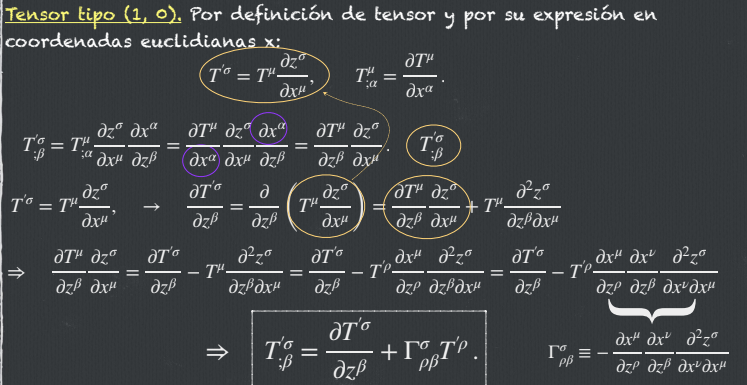
\includegraphics[width=0.95\textwidth]{tensor10.png}
  \end{center}
\end{figure}

\section{Curvatura y torsión }
En $ \mathbb{R}^ {n } $ en coordenadas cartesianas: 
\begin{gather*}
  (\grad _\alpha \grad _{\beta}  - \grad _\beta \grad_\alpha) T _{(\nu )} ^ {(\mu )} = 0  
\end{gather*}
En una variedad general con una conexión arbitraria en general tendremos: 
\begin{gather*}
  (\grad _\alpha \grad _{\beta}  - \grad _\beta \grad_\alpha) T _{(\nu )} ^ {(\mu )} \neq 0  
\end{gather*}

\caja{green}{}{
  \textbf{Tensor de torsión }
  \begin{gather*}
    T(X,Y) = \grad_X Y - \grad_Y X - [X,Y] 
  \end{gather*}
  \textbf{Tensor de ...}
}

\end{document}
